\section{Interval Scheduling Problem}

\subsection*{The Problem}

Given an array of \emph{intervals} $A[1\cdots n]$, where $A[i] = (s(i),t(i))$ is an interval represented with
\emph{start-time} $s(i)$ and \emph{finish-time} $t(i)$, we seek a \emph{compatible} subset $X\subset A$
such that $|X|$ is maximized. Here, $X$ is \emph{compatible} is defined as that intervals in $X$
are disjoint~(i.e., any two intervals in $X$ don't overlap).
See Figure~\ref{fig:interval}.

\begin{figure}[h]
\centering{

\tikzset{every picture/.style={line width=0.75pt}} %set default line width to 0.75pt        

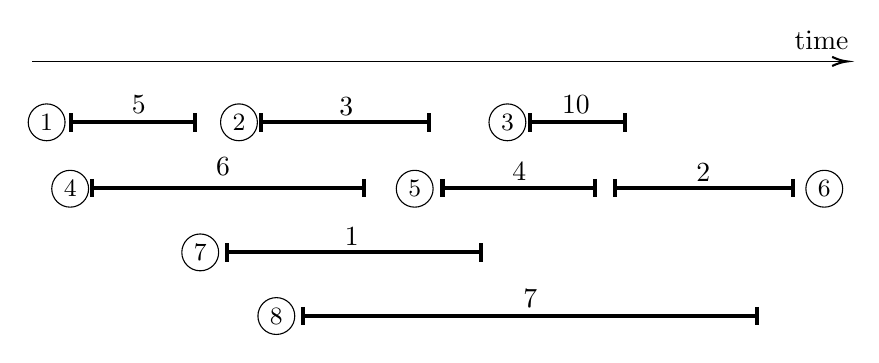
\begin{tikzpicture}[x=0.5pt,y=0.5pt,yscale=-1,xscale=1]
%uncomment if require: \path (0,248); %set diagram left start at 0, and has height of 248

%Straight Lines [id:da9015649955021968] 
\draw    (7,37) -- (594,37) ;
\draw [shift={(596,37)}, rotate = 180] [color={rgb, 255:red, 0; green, 0; blue, 0 }  ][line width=0.75]    (10.93,-3.29) .. controls (6.95,-1.4) and (3.31,-0.3) .. (0,0) .. controls (3.31,0.3) and (6.95,1.4) .. (10.93,3.29)   ;
%Straight Lines [id:da9640237890291299] 
\draw [line width=1.5]    (35,81) -- (124.5,81) ;
\draw [shift={(124.5,81)}, rotate = 180] [color={rgb, 255:red, 0; green, 0; blue, 0 }  ][line width=1.5]    (0,6.71) -- (0,-6.71)   ;
\draw [shift={(35,81)}, rotate = 180] [color={rgb, 255:red, 0; green, 0; blue, 0 }  ][line width=1.5]    (0,6.71) -- (0,-6.71)   ;
%Straight Lines [id:da3355888679808179] 
\draw [line width=1.5]    (172,81) -- (293.5,81) ;
\draw [shift={(293.5,81)}, rotate = 180] [color={rgb, 255:red, 0; green, 0; blue, 0 }  ][line width=1.5]    (0,6.71) -- (0,-6.71)   ;
\draw [shift={(172,81)}, rotate = 180] [color={rgb, 255:red, 0; green, 0; blue, 0 }  ][line width=1.5]    (0,6.71) -- (0,-6.71)   ;
%Straight Lines [id:da09988799250468405] 
\draw [line width=1.5]    (367,81) -- (435.5,81) ;
\draw [shift={(435.5,81)}, rotate = 180] [color={rgb, 255:red, 0; green, 0; blue, 0 }  ][line width=1.5]    (0,6.71) -- (0,-6.71)   ;
\draw [shift={(367,81)}, rotate = 180] [color={rgb, 255:red, 0; green, 0; blue, 0 }  ][line width=1.5]    (0,6.71) -- (0,-6.71)   ;
%Straight Lines [id:da4026459071674142] 
\draw [line width=1.5]    (50,128.5) -- (246.5,128.5) ;
\draw [shift={(246.5,128.5)}, rotate = 180] [color={rgb, 255:red, 0; green, 0; blue, 0 }  ][line width=1.5]    (0,6.71) -- (0,-6.71)   ;
\draw [shift={(50,128.5)}, rotate = 180] [color={rgb, 255:red, 0; green, 0; blue, 0 }  ][line width=1.5]    (0,6.71) -- (0,-6.71)   ;
%Straight Lines [id:da5509115882034084] 
\draw [line width=1.5]    (303.5,128.5) -- (413.5,128.5) ;
\draw [shift={(413.5,128.5)}, rotate = 180] [color={rgb, 255:red, 0; green, 0; blue, 0 }  ][line width=1.5]    (0,6.71) -- (0,-6.71)   ;
\draw [shift={(303.5,128.5)}, rotate = 180] [color={rgb, 255:red, 0; green, 0; blue, 0 }  ][line width=1.5]    (0,6.71) -- (0,-6.71)   ;
%Straight Lines [id:da6271509388583772] 
\draw [line width=1.5]    (428,128.5) -- (556.5,128.5) ;
\draw [shift={(556.5,128.5)}, rotate = 180] [color={rgb, 255:red, 0; green, 0; blue, 0 }  ][line width=1.5]    (0,6.71) -- (0,-6.71)   ;
\draw [shift={(428,128.5)}, rotate = 180] [color={rgb, 255:red, 0; green, 0; blue, 0 }  ][line width=1.5]    (0,6.71) -- (0,-6.71)   ;
%Straight Lines [id:da26802882985941956] 
\draw [line width=1.5]    (147.5,175) -- (331,175) ;
\draw [shift={(331,175)}, rotate = 180] [color={rgb, 255:red, 0; green, 0; blue, 0 }  ][line width=1.5]    (0,6.71) -- (0,-6.71)   ;
\draw [shift={(147.5,175)}, rotate = 180] [color={rgb, 255:red, 0; green, 0; blue, 0 }  ][line width=1.5]    (0,6.71) -- (0,-6.71)   ;
%Straight Lines [id:da22029647624095072] 
\draw [line width=1.5]    (202.5,221) -- (531,221) ;
\draw [shift={(531,221)}, rotate = 180] [color={rgb, 255:red, 0; green, 0; blue, 0 }  ][line width=1.5]    (0,6.71) -- (0,-6.71)   ;
\draw [shift={(202.5,221)}, rotate = 180] [color={rgb, 255:red, 0; green, 0; blue, 0 }  ][line width=1.5]    (0,6.71) -- (0,-6.71)   ;

% Text Node
\draw (556,13) node [anchor=north west][inner sep=0.75pt]   [align=left] {time};
% Text Node
\draw    (17.38, 81) circle [x radius= 13.31, y radius= 13.31]   ;
\draw (17.38,81) node  [font=\small] [align=left] {$\displaystyle 1$};
% Text Node
\draw    (156.38, 81) circle [x radius= 13.31, y radius= 13.31]   ;
\draw (156.38,81) node  [font=\small] [align=left] {$\displaystyle 2$};
% Text Node
\draw    (350.38, 81) circle [x radius= 13.31, y radius= 13.31]   ;
\draw (350.38,81) node  [font=\small] [align=left] {$\displaystyle 3$};
% Text Node
\draw    (34.38, 129) circle [x radius= 13.31, y radius= 13.31]   ;
\draw (34.38,129) node  [font=\small] [align=left] {$\displaystyle 4$};
% Text Node
\draw    (283.38, 129) circle [x radius= 13.31, y radius= 13.31]   ;
\draw (283.38,129) node  [font=\small] [align=left] {$\displaystyle 5$};
% Text Node
\draw    (579.38, 129) circle [x radius= 13.31, y radius= 13.31]   ;
\draw (579.38,129) node  [font=\small] [align=left] {$\displaystyle 6$};
% Text Node
\draw    (128.38, 175) circle [x radius= 13.31, y radius= 13.31]   ;
\draw (128.38,175) node  [font=\small] [align=left] {$\displaystyle 7$};
% Text Node
\draw    (183.38, 221) circle [x radius= 13.31, y radius= 13.31]   ;
\draw (183.38,221) node  [font=\small] [align=left] {$\displaystyle 8$};
% Text Node
\draw (77,60) node [anchor=north west][inner sep=0.75pt]   [align=left] {$\displaystyle 5$};
% Text Node
\draw (227,61) node [anchor=north west][inner sep=0.75pt]   [align=left] {$\displaystyle 3$};
% Text Node
\draw (388,60) node [anchor=north west][inner sep=0.75pt]   [align=left] {$\displaystyle 10$};
% Text Node
\draw (138,105) node [anchor=north west][inner sep=0.75pt]   [align=left] {$\displaystyle 6$};
% Text Node
\draw (352,108) node [anchor=north west][inner sep=0.75pt]   [align=left] {$\displaystyle 4$};
% Text Node
\draw (485,109) node [anchor=north west][inner sep=0.75pt]   [align=left] {$\displaystyle 2$};
% Text Node
\draw (231,155) node [anchor=north west][inner sep=0.75pt]   [align=left] {$\displaystyle 1$};
% Text Node
\draw (360,200) node [anchor=north west][inner sep=0.75pt]   [align=left] {$\displaystyle 7$};


\end{tikzpicture}

}
\caption{An instance of interval scheduling problem.
The optimal solution includes 4 intervals $\{1, 2, 5, 6\}$.}
\label{fig:interval}
\end{figure}

\subsection*{The Algorithm}

Let's design a greedy algorithm for above interval scheduling problem.
Recall that a greedy algorithm iteratively makes \emph{local decisions},
until reaches a complete solution. In particular, for this problem
a greedy algorithm follows the following framework.

\begin{minipage}{0.8\textwidth}
	\aaA {6}{Algorithm greedy-framework~(intervals $A[1\cdots n]$)}\xxx
	\aab {init $X=\emptyset$;}\xxx
	\aaB {3}{while~(true)}\xxx
	\aac {\textcolor{blue}{greedily pick a (new) interval $x\in A$ that doesn't conflict with intervals in $X$} and add it to $X$;}\xxx
	\aac {the algorithm terminates and returns $X$ if such $x$ cannot be found;}\xxx
	\aab {end;}\xxx
	\aaa {end;}\xxx
\end{minipage}

Above procedure is a framework, as how to \emph{greedily pick a new interval that is compatible with $X$} is not specified.
A common practice in order to design a correct~(i.e., optimal) greedy algorithm is
exploring different greedy strategies. For each strategy, we first try to
design a counter-example to show it doesn't work; if such an instance
is hard to construct, then it's a promising direction and we then try to prove that it is optimal.
For this interval scheduling problem, we can explore the following strategies:

\vspace*{-\topsep}
\begin{enumerate}
\item In each iteration, pick the interval with smallest length that is compatible with $X$.
In fact, Figure~\ref{fig:interval}
is an counter-example, where this greedy strategy finds intervals $\{3, 1, 2\}$.
\item In each iteration, pick the interval with fewest conflicts that is compatible with $X$.
You may notice that this strategy actually finds the optimal solution on Figure~\ref{fig:interval}.
But it cannot guarantee optimality on all instances. Can you design an counter-example?
Figure~4.1~(c) of the textbook~[KT], page 117, gives such a counter-example.
\item In each iteration, pick the interval with earliest start-time that is compatible with $X$.
In fact, Figure~\ref{fig:interval} again is an counter-example, where this greedy strategy finds intervals $\{1, 7\}$.
\item In each iteration, pick the interval with earliest finish-time that is compatible with $X$.
You may notice that this strategy also finds the optimal solution on Figure~\ref{fig:interval}.
In fact, this strategy is indeed optimal~(see the formal proof below).
\end{enumerate}

\subsection*{Correctness}

We now show that, the greedy strategy of picking the (compatible) interval with earliest finish-time leads
to an optimal greedy algorithm. First, note that this greedy framework guarantees 
that $X$ is compatible~(even if using the first 3 strategies),
as any newly added interval doesn't overlap with existings ones in $X$.

Now we show that the algorithm is optimal, i.e., $|X|$ is maximized.
Assume that $X = \{A[x_1], A[x_2], \cdots, A[x_k]\}$.
We also assume that these $k$ intervals are sorted by their finish-time, i.e., $t(x_1) \le t(x_2) \le \cdots \le t(x_k)$.
Assume that $X^* = \{A[x^*_1], A[x^*_2], \cdots, A[x^*_m]\}$ be an optimal solution~(with $m$ intervals).
We also assume that these $m$ intervals are sorted by their finish-time, i.e., $t(x^*_1) \le t(x^*_2) \le \cdots \le t(x^*_m)$.

Clearly $k \le m$, as we assume $X^*$ is the optimal solution.
The ultimate goal is to prove that $k = m$, i.e., the greedy algorithm always finds the
same number of intervals with the optimal solution.
In order to achieve it, we first prove a more informative fact,
which shows that the greedy solution always \emph{stays ahead}
of the optimal solution. Specifically,
the finish-time of the $i$-th interval in the greedy solution
is always no latter than the finish-time of the $i$-th interval of the optimal solution,
formally stated below.

\begin{fact} \label{fact1}
For any $1 \le i \le k$, we have $t(x_i) \le t(x_i^*)$.
\end{fact}

\emph{Proof.} We prove it by induction. The base case
is to show $t(x_1) \le t(x_1^*)$. This is obvious,
as the first interval picked by the greedy algorithm 
is always the one with smallest finish-time.

We now show the inductive step. Suppose $t(x_j) \le t(x_j^*)$ for all $1\le j \le i$.
We aim to prove $t(x_{i+1}) \le t(x_{i+1}^*)$. See Figure~\ref{fig:inductive}.
We can write $t(x_i) \le t(x_i^*) \le s(x_{i+1}^*)$. 
This shows that, $A[x^*_{i+1}]$ does not conflict with 
any of these $\{A[x_1], A[x_2], \cdots, A[x_i]\}$.
Hence, when greedy algorithm picks the $(i+1)$-th interval, 
$A[x^*_{i+1}]$ is one of the legitimate candidates.
As the greedy algorithm always pick the one with earliest finish-time~(among all legitimate ones), 
either $A[x^*_{i+1}]$ is picked, or another one with even smaller finish-time~(than $A[x^*_{i+1}]$) is picked;
in either case, we have $t(x_{i+1}) \le t(x_{i+1}^*)$, as desired. \qed

\begin{figure}[h]
\centering{

\tikzset{every picture/.style={line width=0.75pt}} %set default line width to 0.75pt        

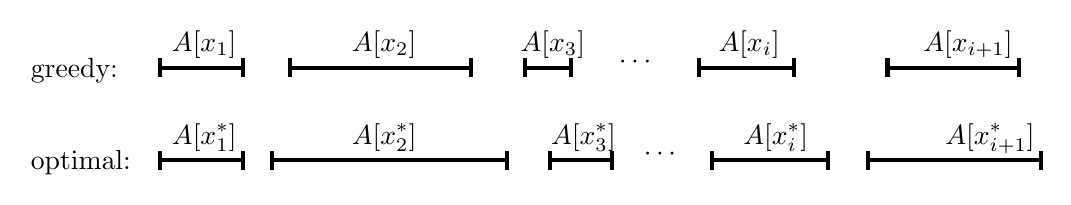
\begin{tikzpicture}[x=0.5pt,y=0.5pt,yscale=-1,xscale=1]
%uncomment if require: \path (0,142); %set diagram left start at 0, and has height of 142

%Straight Lines [id:da9640237890291299] 
\draw [line width=1.5]    (111,47) -- (171.5,47) ;
\draw [shift={(171.5,47)}, rotate = 180] [color={rgb, 255:red, 0; green, 0; blue, 0 }  ][line width=1.5]    (0,6.71) -- (0,-6.71)   ;
\draw [shift={(111,47)}, rotate = 180] [color={rgb, 255:red, 0; green, 0; blue, 0 }  ][line width=1.5]    (0,6.71) -- (0,-6.71)   ;
%Straight Lines [id:da3355888679808179] 
\draw [line width=1.5]    (205,47) -- (336,47) ;
\draw [shift={(336,47)}, rotate = 180] [color={rgb, 255:red, 0; green, 0; blue, 0 }  ][line width=1.5]    (0,6.71) -- (0,-6.71)   ;
\draw [shift={(205,47)}, rotate = 180] [color={rgb, 255:red, 0; green, 0; blue, 0 }  ][line width=1.5]    (0,6.71) -- (0,-6.71)   ;
%Straight Lines [id:da09988799250468405] 
\draw [line width=1.5]    (375,47) -- (408,47) ;
\draw [shift={(408,47)}, rotate = 180] [color={rgb, 255:red, 0; green, 0; blue, 0 }  ][line width=1.5]    (0,6.71) -- (0,-6.71)   ;
\draw [shift={(375,47)}, rotate = 180] [color={rgb, 255:red, 0; green, 0; blue, 0 }  ][line width=1.5]    (0,6.71) -- (0,-6.71)   ;
%Straight Lines [id:da8137923006965678] 
\draw [line width=1.5]    (501,47) -- (569.5,47) ;
\draw [shift={(569.5,47)}, rotate = 180] [color={rgb, 255:red, 0; green, 0; blue, 0 }  ][line width=1.5]    (0,6.71) -- (0,-6.71)   ;
\draw [shift={(501,47)}, rotate = 180] [color={rgb, 255:red, 0; green, 0; blue, 0 }  ][line width=1.5]    (0,6.71) -- (0,-6.71)   ;
%Straight Lines [id:da2017441450503047] 
\draw [line width=1.5]    (637,47) -- (732,47) ;
\draw [shift={(732,47)}, rotate = 180] [color={rgb, 255:red, 0; green, 0; blue, 0 }  ][line width=1.5]    (0,6.71) -- (0,-6.71)   ;
\draw [shift={(637,47)}, rotate = 180] [color={rgb, 255:red, 0; green, 0; blue, 0 }  ][line width=1.5]    (0,6.71) -- (0,-6.71)   ;
%Straight Lines [id:da517279355434781] 
\draw [line width=1.5]    (111,114) -- (171.5,114) ;
\draw [shift={(171.5,114)}, rotate = 180] [color={rgb, 255:red, 0; green, 0; blue, 0 }  ][line width=1.5]    (0,6.71) -- (0,-6.71)   ;
\draw [shift={(111,114)}, rotate = 180] [color={rgb, 255:red, 0; green, 0; blue, 0 }  ][line width=1.5]    (0,6.71) -- (0,-6.71)   ;
%Straight Lines [id:da38986625384521667] 
\draw [line width=1.5]    (192,114) -- (362,114) ;
\draw [shift={(362,114)}, rotate = 180] [color={rgb, 255:red, 0; green, 0; blue, 0 }  ][line width=1.5]    (0,6.71) -- (0,-6.71)   ;
\draw [shift={(192,114)}, rotate = 180] [color={rgb, 255:red, 0; green, 0; blue, 0 }  ][line width=1.5]    (0,6.71) -- (0,-6.71)   ;
%Straight Lines [id:da05974740127099276] 
\draw [line width=1.5]    (393,114) -- (438,114) ;
\draw [shift={(438,114)}, rotate = 180] [color={rgb, 255:red, 0; green, 0; blue, 0 }  ][line width=1.5]    (0,6.71) -- (0,-6.71)   ;
\draw [shift={(393,114)}, rotate = 180] [color={rgb, 255:red, 0; green, 0; blue, 0 }  ][line width=1.5]    (0,6.71) -- (0,-6.71)   ;
%Straight Lines [id:da16736606457108671] 
\draw [line width=1.5]    (510,114) -- (594,114) ;
\draw [shift={(594,114)}, rotate = 180] [color={rgb, 255:red, 0; green, 0; blue, 0 }  ][line width=1.5]    (0,6.71) -- (0,-6.71)   ;
\draw [shift={(510,114)}, rotate = 180] [color={rgb, 255:red, 0; green, 0; blue, 0 }  ][line width=1.5]    (0,6.71) -- (0,-6.71)   ;
%Straight Lines [id:da6988626492100889] 
\draw [line width=1.5]    (623,114) -- (748,114) ;
\draw [shift={(748,114)}, rotate = 180] [color={rgb, 255:red, 0; green, 0; blue, 0 }  ][line width=1.5]    (0,6.71) -- (0,-6.71)   ;
\draw [shift={(623,114)}, rotate = 180] [color={rgb, 255:red, 0; green, 0; blue, 0 }  ][line width=1.5]    (0,6.71) -- (0,-6.71)   ;

% Text Node
\draw (16,38) node [anchor=north west][inner sep=0.75pt]   [align=left] {greedy:};
% Text Node
\draw (118,18.5) node [anchor=north west][inner sep=0.75pt]   [align=left] {$\displaystyle A[ x_{1}$]};
% Text Node
\draw (248,18.5) node [anchor=north west][inner sep=0.75pt]   [align=left] {$\displaystyle A[ x_{2}$]};
% Text Node
\draw (370,18.5) node [anchor=north west][inner sep=0.75pt]   [align=left] {$\displaystyle A[ x_{3}$]};
% Text Node
\draw (513,18.5) node [anchor=north west][inner sep=0.75pt]   [align=left] {$\displaystyle A[ x_{i}$]};
% Text Node
\draw (661,18.5) node [anchor=north west][inner sep=0.75pt]   [align=left] {$\displaystyle A[ x_{i+1}$]};
% Text Node
\draw (16,105) node [anchor=north west][inner sep=0.75pt]   [align=left] {optimal:};
% Text Node
\draw (118,85.5) node [anchor=north west][inner sep=0.75pt]   [align=left] {$\displaystyle A[ x^{*}_{1}$]};
% Text Node
\draw (248,85.5) node [anchor=north west][inner sep=0.75pt]   [align=left] {$\displaystyle A[ x^{*}_{2}$]};
% Text Node
\draw (392,85.5) node [anchor=north west][inner sep=0.75pt]   [align=left] {$\displaystyle A[ x^{*}_{3}$]};
% Text Node
\draw (531,85.5) node [anchor=north west][inner sep=0.75pt]   [align=left] {$\displaystyle A[ x^{*}_{i}$]};
% Text Node
\draw (677,85.5) node [anchor=north west][inner sep=0.75pt]   [align=left] {$\displaystyle A[ x^{*}_{i+1}$]};
% Text Node
\draw (441,36.5) node [anchor=north west][inner sep=0.75pt]   [align=left] {$\displaystyle \cdots $};
% Text Node
\draw (459,103.5) node [anchor=north west][inner sep=0.75pt]   [align=left] {$\displaystyle \cdots $};


\end{tikzpicture}

}
\caption{Illustrating of proving Fact~\ref{fact1}.}
\label{fig:inductive}
\end{figure}

\begin{fact} \label{fact2}
We have $k = m$.
\end{fact}

\emph{Proof.} We prove it by contradiction.
See Figure~\ref{fig:fact2}.  Suppose conversely that $m \ge k + 1$.
Using the same reasong in proving Fact~\ref{fact1},
we know that after picking $\{A[x_1], A[x_2], \cdots, A[x_k]\}$ in the greedy algorithm,
$A[x^*_{i+1}]$ remains legitimate, as it does not overlap with any of these $k$ intervals that are already picked.
Hence, the greedy algorithm won't terminate and will continue to pick at least one more interval.
This contradicts to the assumption that the greedy solution includes $k$ intervals. \qed

\begin{figure}[h]
\centering{

\tikzset{every picture/.style={line width=0.75pt}} %set default line width to 0.75pt        

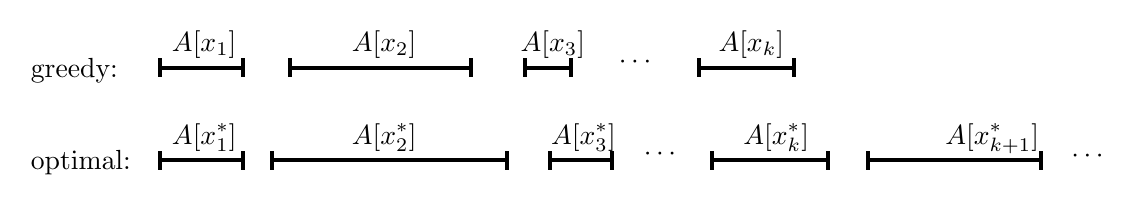
\begin{tikzpicture}[x=0.5pt,y=0.5pt,yscale=-1,xscale=1]
%uncomment if require: \path (0,142); %set diagram left start at 0, and has height of 142

%Straight Lines [id:da9640237890291299] 
\draw [line width=1.5]    (111,47) -- (171.5,47) ;
\draw [shift={(171.5,47)}, rotate = 180] [color={rgb, 255:red, 0; green, 0; blue, 0 }  ][line width=1.5]    (0,6.71) -- (0,-6.71)   ;
\draw [shift={(111,47)}, rotate = 180] [color={rgb, 255:red, 0; green, 0; blue, 0 }  ][line width=1.5]    (0,6.71) -- (0,-6.71)   ;
%Straight Lines [id:da3355888679808179] 
\draw [line width=1.5]    (205,47) -- (336,47) ;
\draw [shift={(336,47)}, rotate = 180] [color={rgb, 255:red, 0; green, 0; blue, 0 }  ][line width=1.5]    (0,6.71) -- (0,-6.71)   ;
\draw [shift={(205,47)}, rotate = 180] [color={rgb, 255:red, 0; green, 0; blue, 0 }  ][line width=1.5]    (0,6.71) -- (0,-6.71)   ;
%Straight Lines [id:da09988799250468405] 
\draw [line width=1.5]    (375,47) -- (408,47) ;
\draw [shift={(408,47)}, rotate = 180] [color={rgb, 255:red, 0; green, 0; blue, 0 }  ][line width=1.5]    (0,6.71) -- (0,-6.71)   ;
\draw [shift={(375,47)}, rotate = 180] [color={rgb, 255:red, 0; green, 0; blue, 0 }  ][line width=1.5]    (0,6.71) -- (0,-6.71)   ;
%Straight Lines [id:da8137923006965678] 
\draw [line width=1.5]    (501,47) -- (569.5,47) ;
\draw [shift={(569.5,47)}, rotate = 180] [color={rgb, 255:red, 0; green, 0; blue, 0 }  ][line width=1.5]    (0,6.71) -- (0,-6.71)   ;
\draw [shift={(501,47)}, rotate = 180] [color={rgb, 255:red, 0; green, 0; blue, 0 }  ][line width=1.5]    (0,6.71) -- (0,-6.71)   ;
%Straight Lines [id:da517279355434781] 
\draw [line width=1.5]    (111,114) -- (171.5,114) ;
\draw [shift={(171.5,114)}, rotate = 180] [color={rgb, 255:red, 0; green, 0; blue, 0 }  ][line width=1.5]    (0,6.71) -- (0,-6.71)   ;
\draw [shift={(111,114)}, rotate = 180] [color={rgb, 255:red, 0; green, 0; blue, 0 }  ][line width=1.5]    (0,6.71) -- (0,-6.71)   ;
%Straight Lines [id:da38986625384521667] 
\draw [line width=1.5]    (192,114) -- (362,114) ;
\draw [shift={(362,114)}, rotate = 180] [color={rgb, 255:red, 0; green, 0; blue, 0 }  ][line width=1.5]    (0,6.71) -- (0,-6.71)   ;
\draw [shift={(192,114)}, rotate = 180] [color={rgb, 255:red, 0; green, 0; blue, 0 }  ][line width=1.5]    (0,6.71) -- (0,-6.71)   ;
%Straight Lines [id:da05974740127099276] 
\draw [line width=1.5]    (393,114) -- (438,114) ;
\draw [shift={(438,114)}, rotate = 180] [color={rgb, 255:red, 0; green, 0; blue, 0 }  ][line width=1.5]    (0,6.71) -- (0,-6.71)   ;
\draw [shift={(393,114)}, rotate = 180] [color={rgb, 255:red, 0; green, 0; blue, 0 }  ][line width=1.5]    (0,6.71) -- (0,-6.71)   ;
%Straight Lines [id:da16736606457108671] 
\draw [line width=1.5]    (510,114) -- (594,114) ;
\draw [shift={(594,114)}, rotate = 180] [color={rgb, 255:red, 0; green, 0; blue, 0 }  ][line width=1.5]    (0,6.71) -- (0,-6.71)   ;
\draw [shift={(510,114)}, rotate = 180] [color={rgb, 255:red, 0; green, 0; blue, 0 }  ][line width=1.5]    (0,6.71) -- (0,-6.71)   ;
%Straight Lines [id:da6988626492100889] 
\draw [line width=1.5]    (623,114) -- (748,114) ;
\draw [shift={(748,114)}, rotate = 180] [color={rgb, 255:red, 0; green, 0; blue, 0 }  ][line width=1.5]    (0,6.71) -- (0,-6.71)   ;
\draw [shift={(623,114)}, rotate = 180] [color={rgb, 255:red, 0; green, 0; blue, 0 }  ][line width=1.5]    (0,6.71) -- (0,-6.71)   ;

% Text Node
\draw (16,38) node [anchor=north west][inner sep=0.75pt]   [align=left] {greedy:};
% Text Node
\draw (118,18.5) node [anchor=north west][inner sep=0.75pt]   [align=left] {$\displaystyle A[ x_{1}$]};
% Text Node
\draw (248,18.5) node [anchor=north west][inner sep=0.75pt]   [align=left] {$\displaystyle A[ x_{2}$]};
% Text Node
\draw (370,18.5) node [anchor=north west][inner sep=0.75pt]   [align=left] {$\displaystyle A[ x_{3}$]};
% Text Node
\draw (513,18.5) node [anchor=north west][inner sep=0.75pt]   [align=left] {$\displaystyle A[ x_{k}$]};
% Text Node
\draw (16,105) node [anchor=north west][inner sep=0.75pt]   [align=left] {optimal:};
% Text Node
\draw (118,85.5) node [anchor=north west][inner sep=0.75pt]   [align=left] {$\displaystyle A[ x^{*}_{1}$]};
% Text Node
\draw (248,85.5) node [anchor=north west][inner sep=0.75pt]   [align=left] {$\displaystyle A[ x^{*}_{2}$]};
% Text Node
\draw (392,85.5) node [anchor=north west][inner sep=0.75pt]   [align=left] {$\displaystyle A[ x^{*}_{3}$]};
% Text Node
\draw (531,85.5) node [anchor=north west][inner sep=0.75pt]   [align=left] {$\displaystyle A[ x^{*}_{k}$]};
% Text Node
\draw (677,85.5) node [anchor=north west][inner sep=0.75pt]   [align=left] {$\displaystyle A[ x^{*}_{k+1}$]};
% Text Node
\draw (441,36.5) node [anchor=north west][inner sep=0.75pt]   [align=left] {$\displaystyle \cdots $};
% Text Node
\draw (459,103.5) node [anchor=north west][inner sep=0.75pt]   [align=left] {$\displaystyle \cdots $};
% Text Node
\draw (768,105) node [anchor=north west][inner sep=0.75pt]   [align=left] {$\displaystyle \cdots $};


\end{tikzpicture}

}
\caption{Illustrating of proving Fact~\ref{fact2}.}
\label{fig:fact2}
\end{figure}


\subsection*{The Complete Algorithm}

How to efficiently pick the interval with earliest finish-time that is compatible with existing ones~(i.e., those in $X$)?
We can sort all intervals by their finish-time, examine them one-by-one following this order, and include it when it does not
conflict with those in $X$---a similar approach is used in the Kruskal's algorithm.
Then in each itertion, how to decide if the current interval is compatible with $X$?
A naive solution is to compare it with all intervals in $X$, but this will take linear time and the resulting algorithm will take $O(n^2)$ time.
In fact, we can do it faster. 
As all intervals are now sorted by their finish-time,
we have that the current interval can be safely added if and only if its start-time
is larger or equal to the finish-time of the previously added interval.
Hence, we simply maintain the last interval that is added to $X$,
and we can use a single comparison, which takes constant time, to decide if the current one is compatible with $X$ or not.

The pseudo-code is given below.
The for-loop takes linear time. The entire algorithm takes $O(n\log n)$ time, as it is dominated by sorting.
An example of running this algorithm follows.

\begin{minipage}{0.8\textwidth}
	\aaA {11}{Algorithm greedy~(intervals $A[1\cdots n]$)}\xxx
	\aab {sort $A$ by their finish-time;}\xxx
	\aab {init $X=\{A[1]\}$;}\xxx
	\aab {let $j=1$;\ \ // maintain the previously added interval}\xxx
	\aaB {5}{for $i = 2 \to n$}\xxx
	\aaC {3}{if~($s(i) \ge t(j)$)}\xxx
	\aad {pick $A[i]$ and add it to $X$;}\xxx
	\aad {$j = i$;}\xxx
	\aac {end;}\xxx
	\aab {end;}\xxx
	\aab {return $X$;}\xxx
	\aaa {end;}\xxx
\end{minipage}

\vspace*{-0.8cm}

\begin{figure}[h]
\centering{

\tikzset{every picture/.style={line width=0.75pt}} %set default line width to 0.75pt        

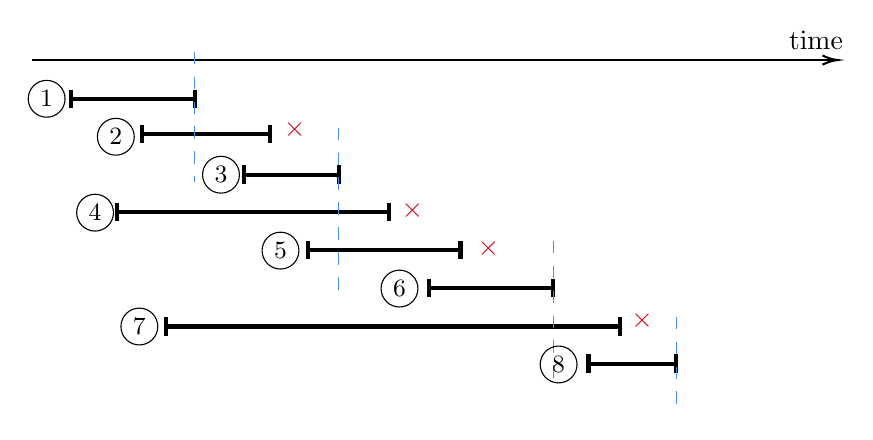
\begin{tikzpicture}[x=0.5pt,y=0.5pt,yscale=-1,xscale=1]
%uncomment if require: \path (0,309); %set diagram left start at 0, and has height of 309

%Straight Lines [id:da9015649955021968] 
\draw    (11,36) -- (591,36) ;
\draw [shift={(593,36)}, rotate = 180] [color={rgb, 255:red, 0; green, 0; blue, 0 }  ][line width=0.75]    (10.93,-3.29) .. controls (6.95,-1.4) and (3.31,-0.3) .. (0,0) .. controls (3.31,0.3) and (6.95,1.4) .. (10.93,3.29)   ;
%Straight Lines [id:da32866075720806565] 
\draw [line width=1.5]    (39,64) -- (128.5,64) ;
\draw [shift={(128.5,64)}, rotate = 180] [color={rgb, 255:red, 0; green, 0; blue, 0 }  ][line width=1.5]    (0,6.71) -- (0,-6.71)   ;
\draw [shift={(39,64)}, rotate = 180] [color={rgb, 255:red, 0; green, 0; blue, 0 }  ][line width=1.5]    (0,6.71) -- (0,-6.71)   ;

%Straight Lines [id:da254468097345411] 
\draw [line width=1.5]    (90.5,89.43) -- (182.5,89.43) ;
\draw [shift={(182.5,89.43)}, rotate = 180] [color={rgb, 255:red, 0; green, 0; blue, 0 }  ][line width=1.5]    (0,6.71) -- (0,-6.71)   ;
\draw [shift={(90.5,89.43)}, rotate = 180] [color={rgb, 255:red, 0; green, 0; blue, 0 }  ][line width=1.5]    (0,6.71) -- (0,-6.71)   ;

%Straight Lines [id:da3468808931598407] 
\draw [line width=1.5]    (164,118.86) -- (232.5,118.86) ;
\draw [shift={(232.5,118.86)}, rotate = 180] [color={rgb, 255:red, 0; green, 0; blue, 0 }  ][line width=1.5]    (0,6.71) -- (0,-6.71)   ;
\draw [shift={(164,118.86)}, rotate = 180] [color={rgb, 255:red, 0; green, 0; blue, 0 }  ][line width=1.5]    (0,6.71) -- (0,-6.71)   ;

%Straight Lines [id:da18209051305473312] 
\draw [line width=1.5]    (72,145.79) -- (268.5,145.79) ;
\draw [shift={(268.5,145.79)}, rotate = 180] [color={rgb, 255:red, 0; green, 0; blue, 0 }  ][line width=1.5]    (0,6.71) -- (0,-6.71)   ;
\draw [shift={(72,145.79)}, rotate = 180] [color={rgb, 255:red, 0; green, 0; blue, 0 }  ][line width=1.5]    (0,6.71) -- (0,-6.71)   ;

%Straight Lines [id:da8863435056826324] 
\draw [line width=1.5]    (210.5,173.22) -- (320.5,173.22) ;
\draw [shift={(320.5,173.22)}, rotate = 180] [color={rgb, 255:red, 0; green, 0; blue, 0 }  ][line width=1.5]    (0,6.71) -- (0,-6.71)   ;
\draw [shift={(210.5,173.22)}, rotate = 180] [color={rgb, 255:red, 0; green, 0; blue, 0 }  ][line width=1.5]    (0,6.71) -- (0,-6.71)   ;

%Straight Lines [id:da8287805623261496] 
\draw [line width=1.5]    (298,200.65) -- (387.5,200.65) ;
\draw [shift={(387.5,200.65)}, rotate = 180] [color={rgb, 255:red, 0; green, 0; blue, 0 }  ][line width=1.5]    (0,6.71) -- (0,-6.71)   ;
\draw [shift={(298,200.65)}, rotate = 180] [color={rgb, 255:red, 0; green, 0; blue, 0 }  ][line width=1.5]    (0,6.71) -- (0,-6.71)   ;

%Straight Lines [id:da032564250121786986] 
\draw [line width=1.5]    (107.5,228.58) -- (436,228.58) ;
\draw [shift={(436,228.58)}, rotate = 180] [color={rgb, 255:red, 0; green, 0; blue, 0 }  ][line width=1.5]    (0,6.71) -- (0,-6.71)   ;
\draw [shift={(107.5,228.58)}, rotate = 180] [color={rgb, 255:red, 0; green, 0; blue, 0 }  ][line width=1.5]    (0,6.71) -- (0,-6.71)   ;

%Straight Lines [id:da39810447379181857] 
\draw [line width=1.5]    (413,255.5) -- (476.5,255.5) ;
\draw [shift={(476.5,255.5)}, rotate = 180] [color={rgb, 255:red, 0; green, 0; blue, 0 }  ][line width=1.5]    (0,6.71) -- (0,-6.71)   ;
\draw [shift={(413,255.5)}, rotate = 180] [color={rgb, 255:red, 0; green, 0; blue, 0 }  ][line width=1.5]    (0,6.71) -- (0,-6.71)   ;

%Straight Lines [id:da46422592981377986] 
\draw [color={rgb, 255:red, 74; green, 144; blue, 226 }  ,draw opacity=1 ] [dash pattern={on 4.5pt off 4.5pt}]  (128.5,30) -- (128.5,124) ;
%Straight Lines [id:da6351884156456712] 
\draw [color={rgb, 255:red, 74; green, 144; blue, 226 }  ,draw opacity=1 ] [dash pattern={on 4.5pt off 4.5pt}]  (232.5,84.86) -- (232.5,202) ;
%Straight Lines [id:da33627378877589575] 
\draw [color={rgb, 255:red, 74; green, 144; blue, 226 }  ,draw opacity=1 ] [dash pattern={on 4.5pt off 4.5pt}]  (387.5,166.65) -- (387.5,273) ;
%Straight Lines [id:da20534568749266735] 
\draw [color={rgb, 255:red, 74; green, 144; blue, 226 }  ,draw opacity=1 ] [dash pattern={on 4.5pt off 4.5pt}]  (476.5,221.5) -- (476.5,289.5) ;

% Text Node
\draw (556,13) node [anchor=north west][inner sep=0.75pt]   [align=left] {time};
% Text Node
\draw    (88.38, 228.58) circle [x radius= 13.31, y radius= 13.31]   ;
\draw (88.38,228.58) node  [font=\small] [align=left] {$\displaystyle 7$};
% Text Node
\draw    (190.38, 173.72) circle [x radius= 13.31, y radius= 13.31]   ;
\draw (190.38,173.72) node  [font=\small] [align=left] {$\displaystyle 5$};
% Text Node
\draw    (56.38, 146.29) circle [x radius= 13.31, y radius= 13.31]   ;
\draw (56.38,146.29) node  [font=\small] [align=left] {$\displaystyle 4$};
% Text Node
\draw    (147.38, 118.86) circle [x radius= 13.31, y radius= 13.31]   ;
\draw (147.38,118.86) node  [font=\small] [align=left] {$\displaystyle 3$};
% Text Node
\draw    (21.38, 64) circle [x radius= 13.31, y radius= 13.31]   ;
\draw (21.38,64) node  [font=\small] [align=left] {$\displaystyle 1$};
% Text Node
\draw    (71.38, 91.43) circle [x radius= 13.31, y radius= 13.31]   ;
\draw (71.38,91.43) node  [font=\small] [align=left] {$\displaystyle 2$};
% Text Node
\draw    (276.38, 201.15) circle [x radius= 13.31, y radius= 13.31]   ;
\draw (276.38,201.15) node  [font=\small] [align=left] {$\displaystyle 6$};
% Text Node
\draw    (391.38, 256) circle [x radius= 13.31, y radius= 13.31]   ;
\draw (391.38,256) node  [font=\small] [align=left] {$\displaystyle 8$};
% Text Node
\draw (138,55) node [anchor=north west][inner sep=0.75pt]   [align=left] {$\displaystyle \textcolor[rgb]{0.29,0.56,0.89}{\checkmark }$};
% Text Node
\draw (191,78) node [anchor=north west][inner sep=0.75pt]   [align=left] {$\displaystyle \textcolor[rgb]{0.82,0.01,0.11}{\times }$};
% Text Node
\draw (276,136) node [anchor=north west][inner sep=0.75pt]   [align=left] {$\displaystyle \textcolor[rgb]{0.82,0.01,0.11}{\times }$};
% Text Node
\draw (331,164) node [anchor=north west][inner sep=0.75pt]   [align=left] {$\displaystyle \textcolor[rgb]{0.82,0.01,0.11}{\times }$};
% Text Node
\draw (442,216) node [anchor=north west][inner sep=0.75pt]   [align=left] {$\displaystyle \textcolor[rgb]{0.82,0.01,0.11}{\times }$};
% Text Node
\draw (244,111) node [anchor=north west][inner sep=0.75pt]   [align=left] {$\displaystyle \textcolor[rgb]{0.29,0.56,0.89}{\checkmark }$};
% Text Node
\draw (400,192) node [anchor=north west][inner sep=0.75pt]   [align=left] {$\displaystyle \textcolor[rgb]{0.29,0.56,0.89}{\checkmark }$};
% Text Node
\draw (486,244) node [anchor=north west][inner sep=0.75pt]   [align=left] {$\displaystyle \textcolor[rgb]{0.29,0.56,0.89}{\checkmark }$};


\end{tikzpicture}

}
\caption{An example of running above algorithm.}
\label{fig:jump}
\end{figure}



